In order to obtain optimal performance from the neural network
given a set of atomistic configurations we need a careful choice of parameters
and neural network architecture. The parameters can be classified as either
\textit{training parameters} - such as learning rate and force loss coefficient -
or \textit{architectural parameters} - such as the number of neurons and hidden layers,
or the choice of interaction cutoff radius. The former are important
in the training of the neural network, i.e. adjusting weights and biases
while the latter influence both the training process and the final
deployment of the neural networks on unfamiliar data.
In this section we will be employing a grid search over a set of
parameters, training multiple neural networks on the same data set
and subsequently testing energy and force Root Mean Squared Errors on
a smaller test data set. Generally we will only be training the neural networks
on the energies, since training with forces is much more CPU- and memory-
intensive. However, training with forces would likely affect the final
result and improve the force RMSEs, as we will observe in the following section.
\par
The parameters are unless otherwise specified the defaults listed
in table \ref{table:defaults}.
In their paper on Random Search, \parencite[Bergstra and Bengio]{
    bergstra2012random}
demonstrate that Random Search outperforms Grid Search for dimensions
of search space larger than 3 or 4. However, since we have tested
a small number of parameters (since training and testing is costly)
and we have a general idea of what parameters are appropriate, we
have chosen to employ Grid Search.
AMP has a built in simulated annealing (see for example \cite{
    bertsimas1993simulated}) module, which performs
simulated annealing on the weights and biases of the network,
in order to find values for which the loss is lowest.
The annealing is run for every trained neural network
for 2000 steps at the beginning of the training procedure,
with temperatures starting at $T_{max} = 20$ and ending with $T_{min} = 1$.
Simulated annealing is a suitable algorithm for finding minima
in a complicated energy landscape, and it reduces somewhat
the randomness of initialization so that the results are comparable
without having to perform many runs.
We will also be using the BFGS Quasi-Newton (see for example \cite{
    bonnans2006numerical}) method implemented
through the \textit{scipy.optimize} library. This is
the optimizer interface currently provided by AMP
and the BFGS optimizer generally performs the best.
Finally we mention that AMP initializes the weights and biases
of the neural network using Xavier initialization\cite{glorot2010understanding},
as we discussed briefly in chapter \ref{chap:optimization}.

\begin{table}[H]
\centering
\begin{tabular}{@{}lll@{}}
\toprule
\multicolumn{3}{l}{Hyperparameters}                                    \\ \midrule
Architecture & Symmetry functions & 12 radial, 20 angular               \\
             & Hidden layers      & (10, 10)                           \\
             & Activation         & Hyperbolic tangent                 \\
             & Cutoff function    & Polynomial, $R_c = 6.0, \gamma = 5.0$
             \\
Training     & Epochs             & 2000                               \\
             & Energy coefficient & 1.0                                \\
             & Force coefficient  & None                                \\
             & Regularization     & $\lambda = 10^{-8}$                \\
             & Optimizer          & BFGS                               \\ \bottomrule
\end{tabular}
\caption{Training default values.}
\label{table:defaults}
\end{table}

The AMP package provides a set of defaults for most elements,
and these symmetry functions are plotted in figure \ref{fig:default}.
However, we did not feel that these covered the radial and angular space
sufficiently so we constructed our own instead which is what we will
use for training. AMP only provides centered radial functions,
while we use a mix of centered and shifted radial functions
since these have demonstrated higher performance, as is discussed
in the section on symmetry functions.
For the symmetry functions we have chosen a set of 6 uncentered radial,
6 centered radial and 20 angular (G4)
symmetry functions.
The uncentered radial functions have $\eta$'s spaced evenly
from 1 to 20 and are centered at 0. The centered radial functions
are centered evenly from 0.5 to $R_c - 0.5$ with $\eta = 5.0$.
The angular functions have $\eta$'s spaced evenly from
0.01 to 3 with $\zeta = 1$ and $\gamma = \pm 1$.
These symmetry functions are displayed in figure \ref{fig:selected}.
We have also chosen to employ the polynomial cutoff introduced in AMP
with $\gamma = 5.0$,
since this has a larger set of values inside the cutoff boundary.
The numerical values of the parameters are available in \ref{chap:appendix-a}.

\begin{figure}[H]
\begin{adjustbox}{max width=1.2\linewidth,center}
\centering
  \begin{subfigure}[b]{0.55\textwidth}
      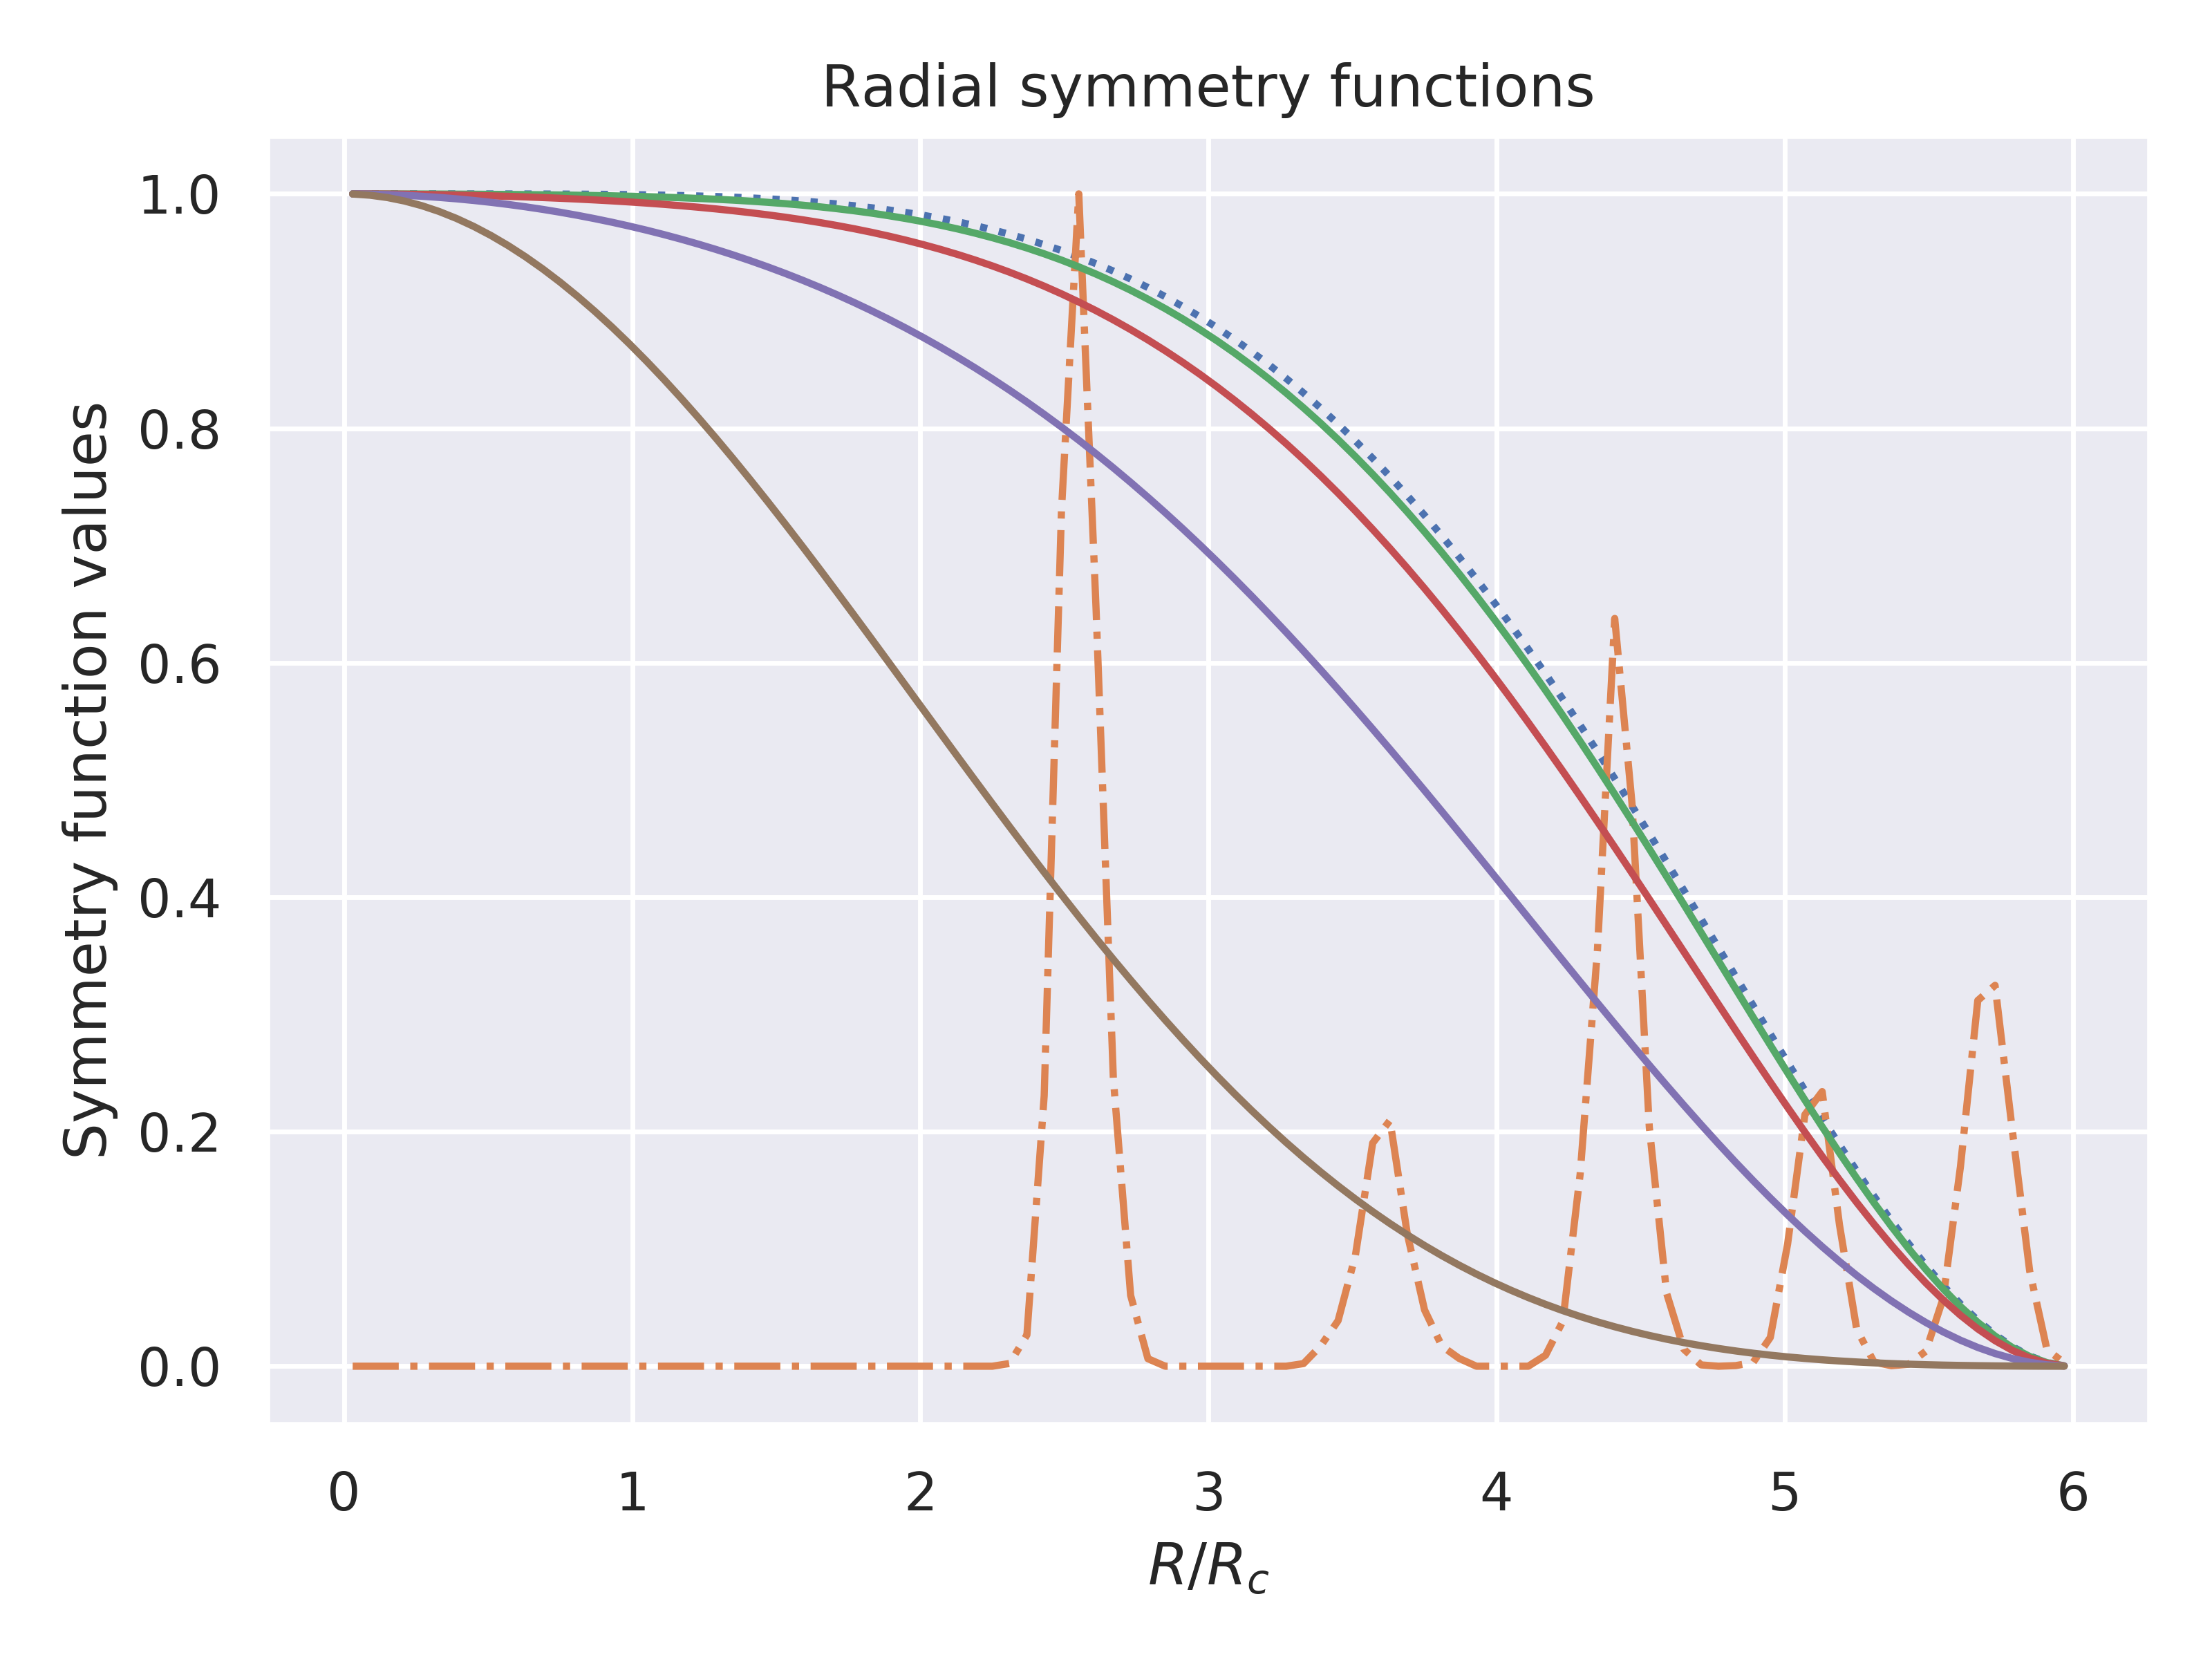
\includegraphics[width=\textwidth]{Default_rad.png}
      \caption{Radial symmetry functions.}
    \label{fig:f1}
  \end{subfigure}
  \hfill
  \begin{subfigure}[b]{0.55\textwidth}
      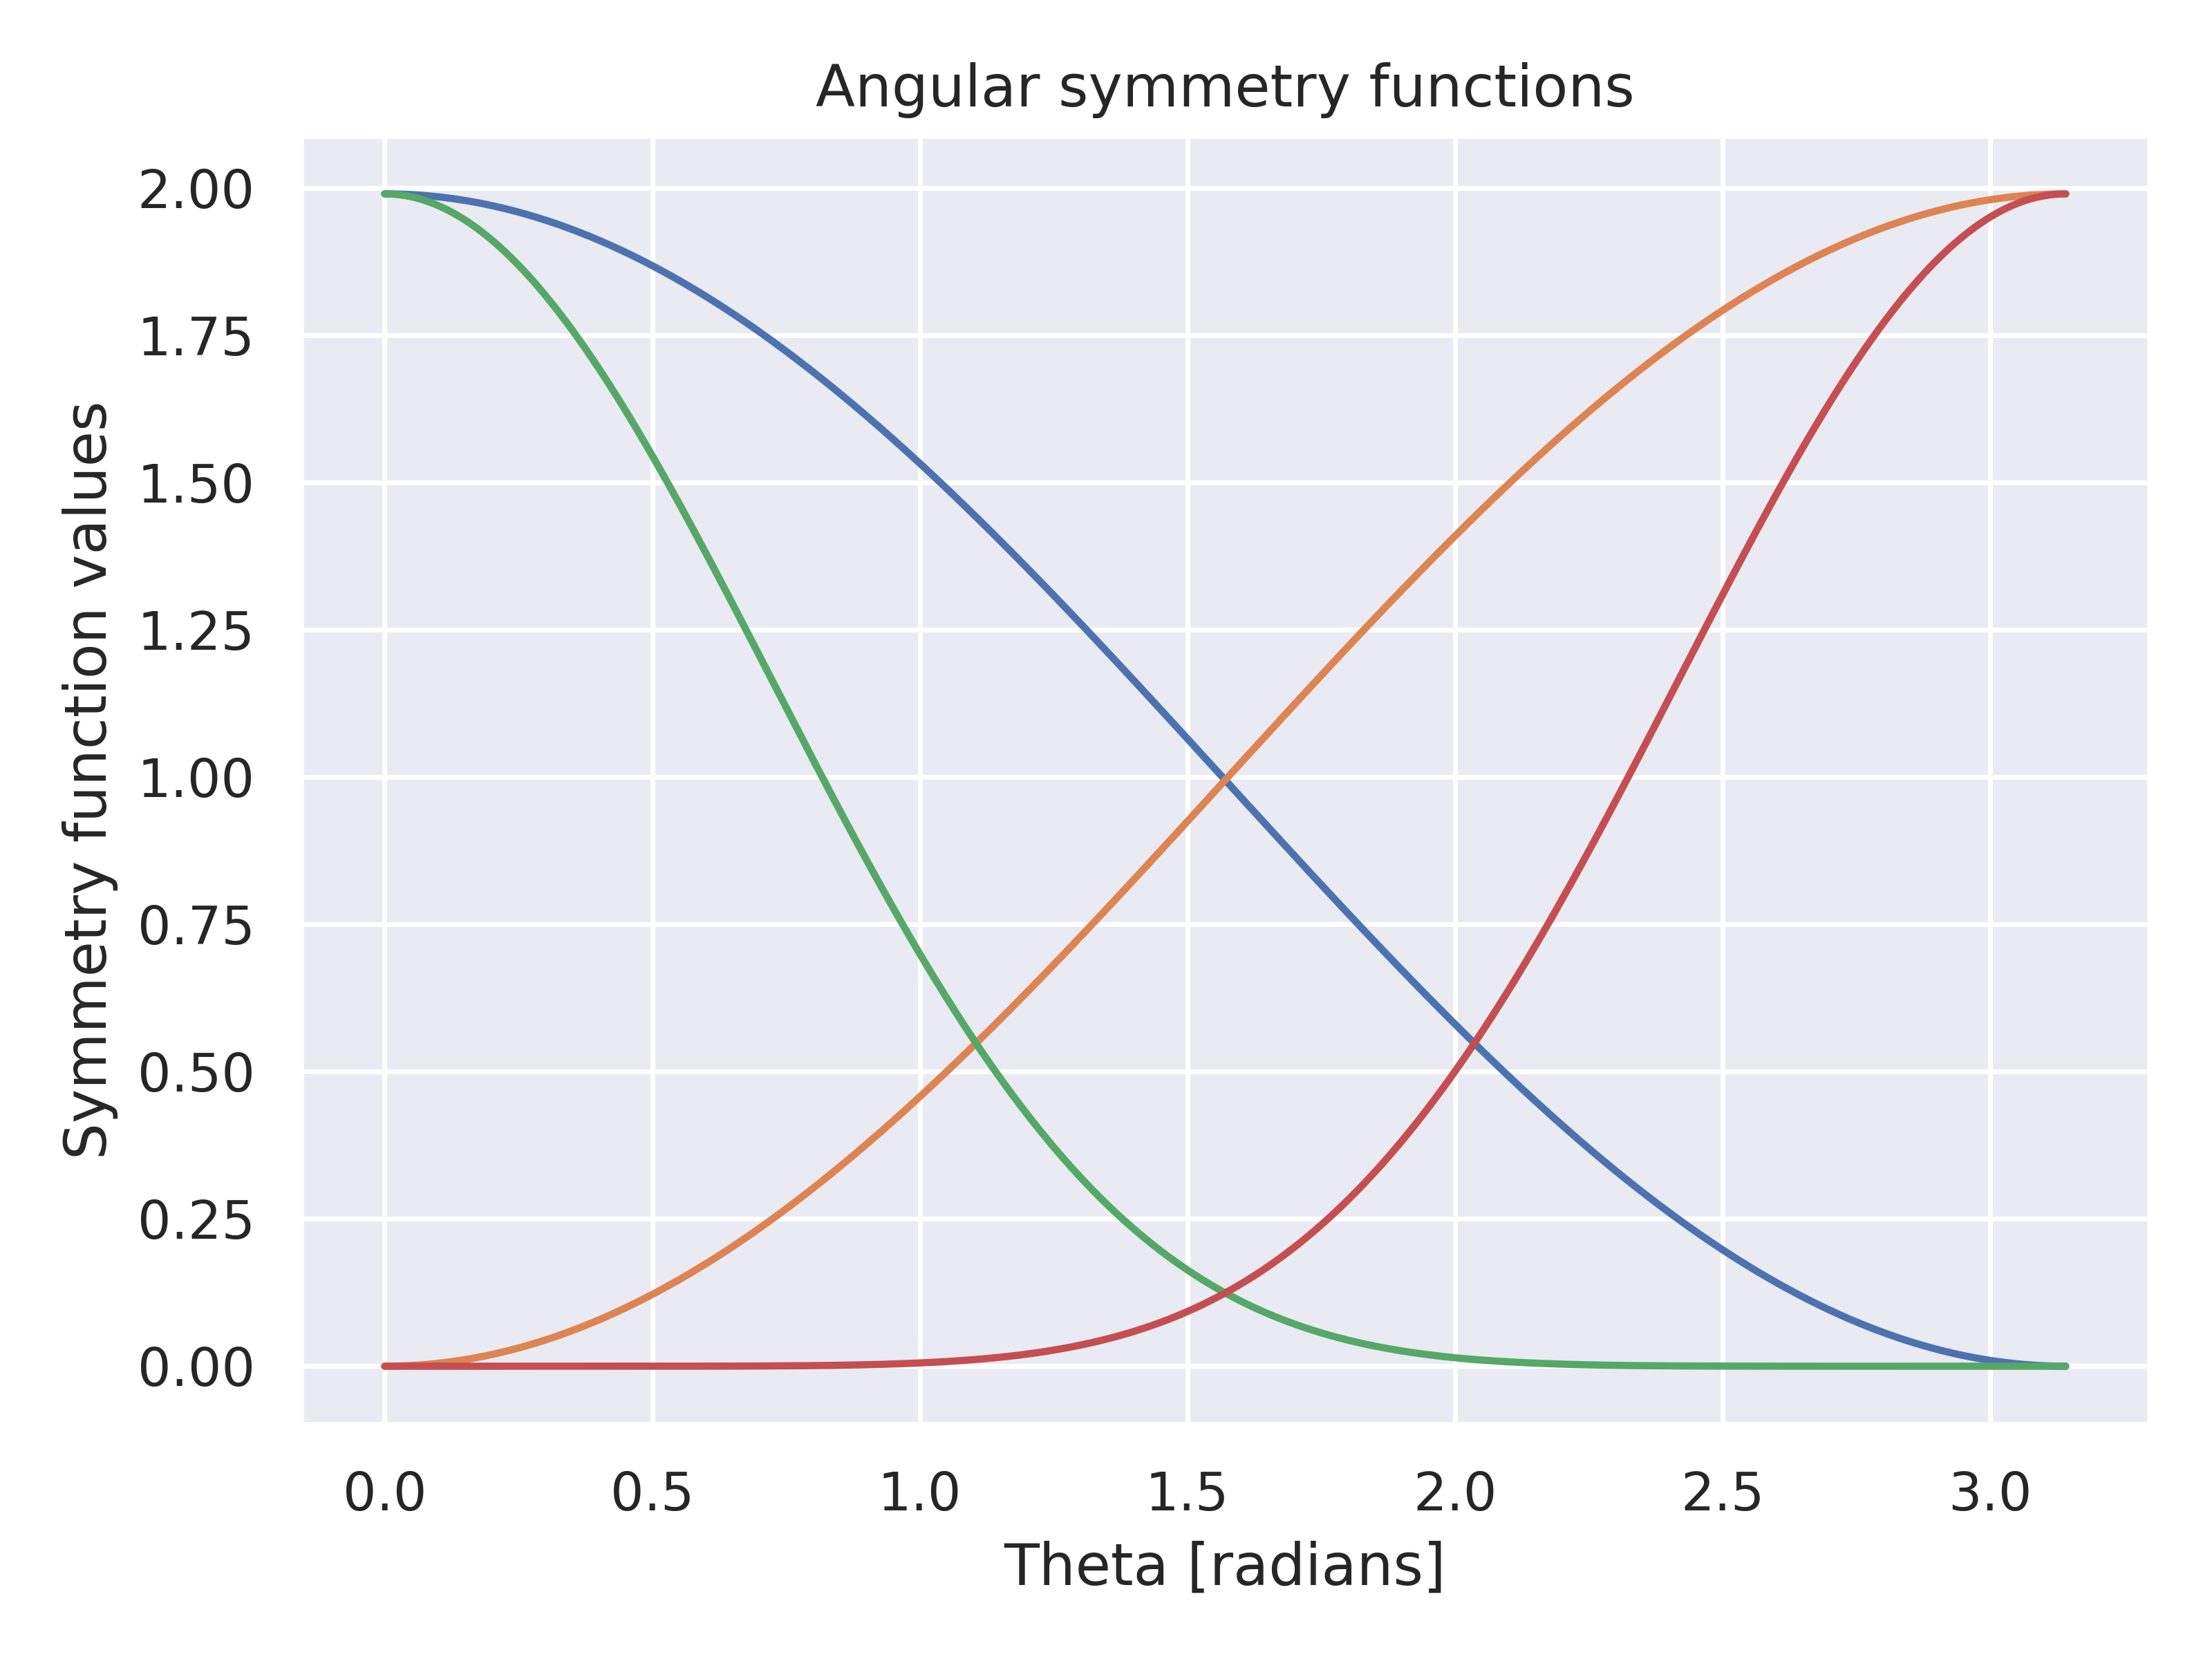
\includegraphics[width=\textwidth]{Default_ang.png}
      \caption{Angular symmetry functions.}
    \label{fig:f2}
  \end{subfigure}
\end{adjustbox}
    \caption{AMP default symmetry function set. Radial functions
    plotted with radial distribution function.}
    \label{fig:default}
\end{figure}

\begin{figure}[H]
\begin{adjustbox}{max width=1.2\linewidth,center}
\centering
  \begin{subfigure}[b]{0.55\textwidth}
      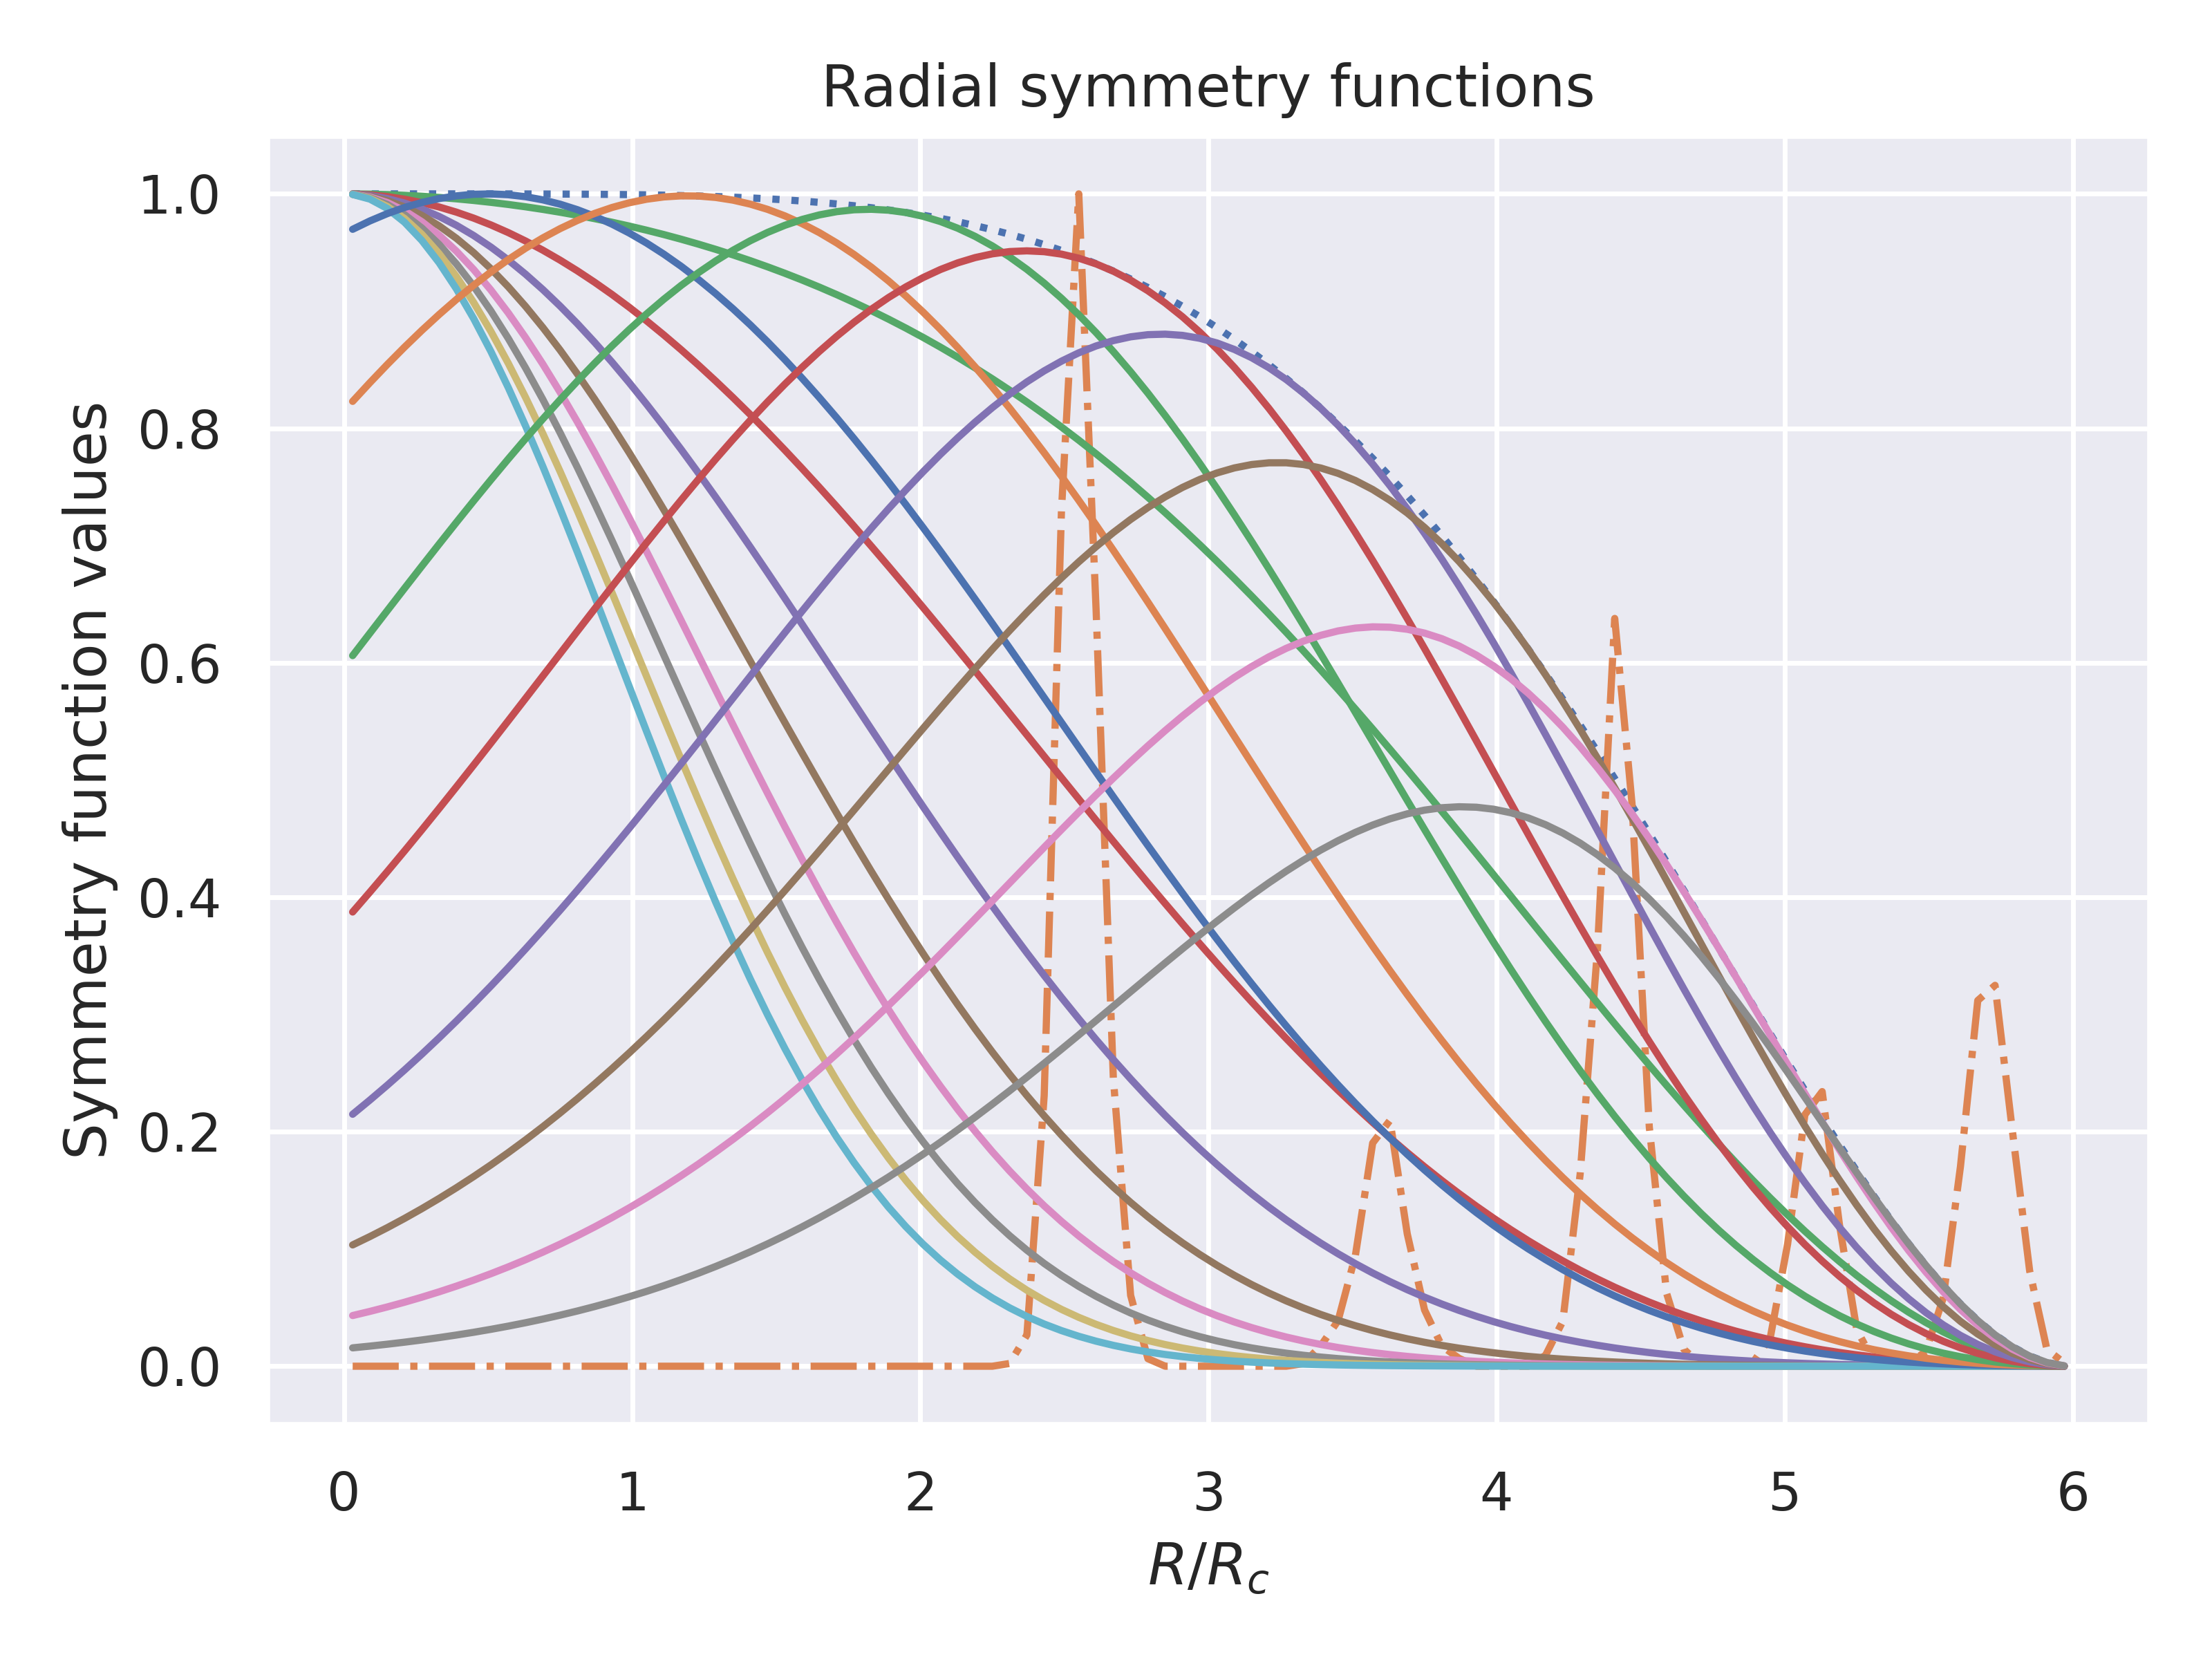
\includegraphics[width=\textwidth]{Selected_rad.png}
      \caption{Radial symmetry functions.}
    \label{fig:f1}
  \end{subfigure}
  \hfill
  \begin{subfigure}[b]{0.55\textwidth}
      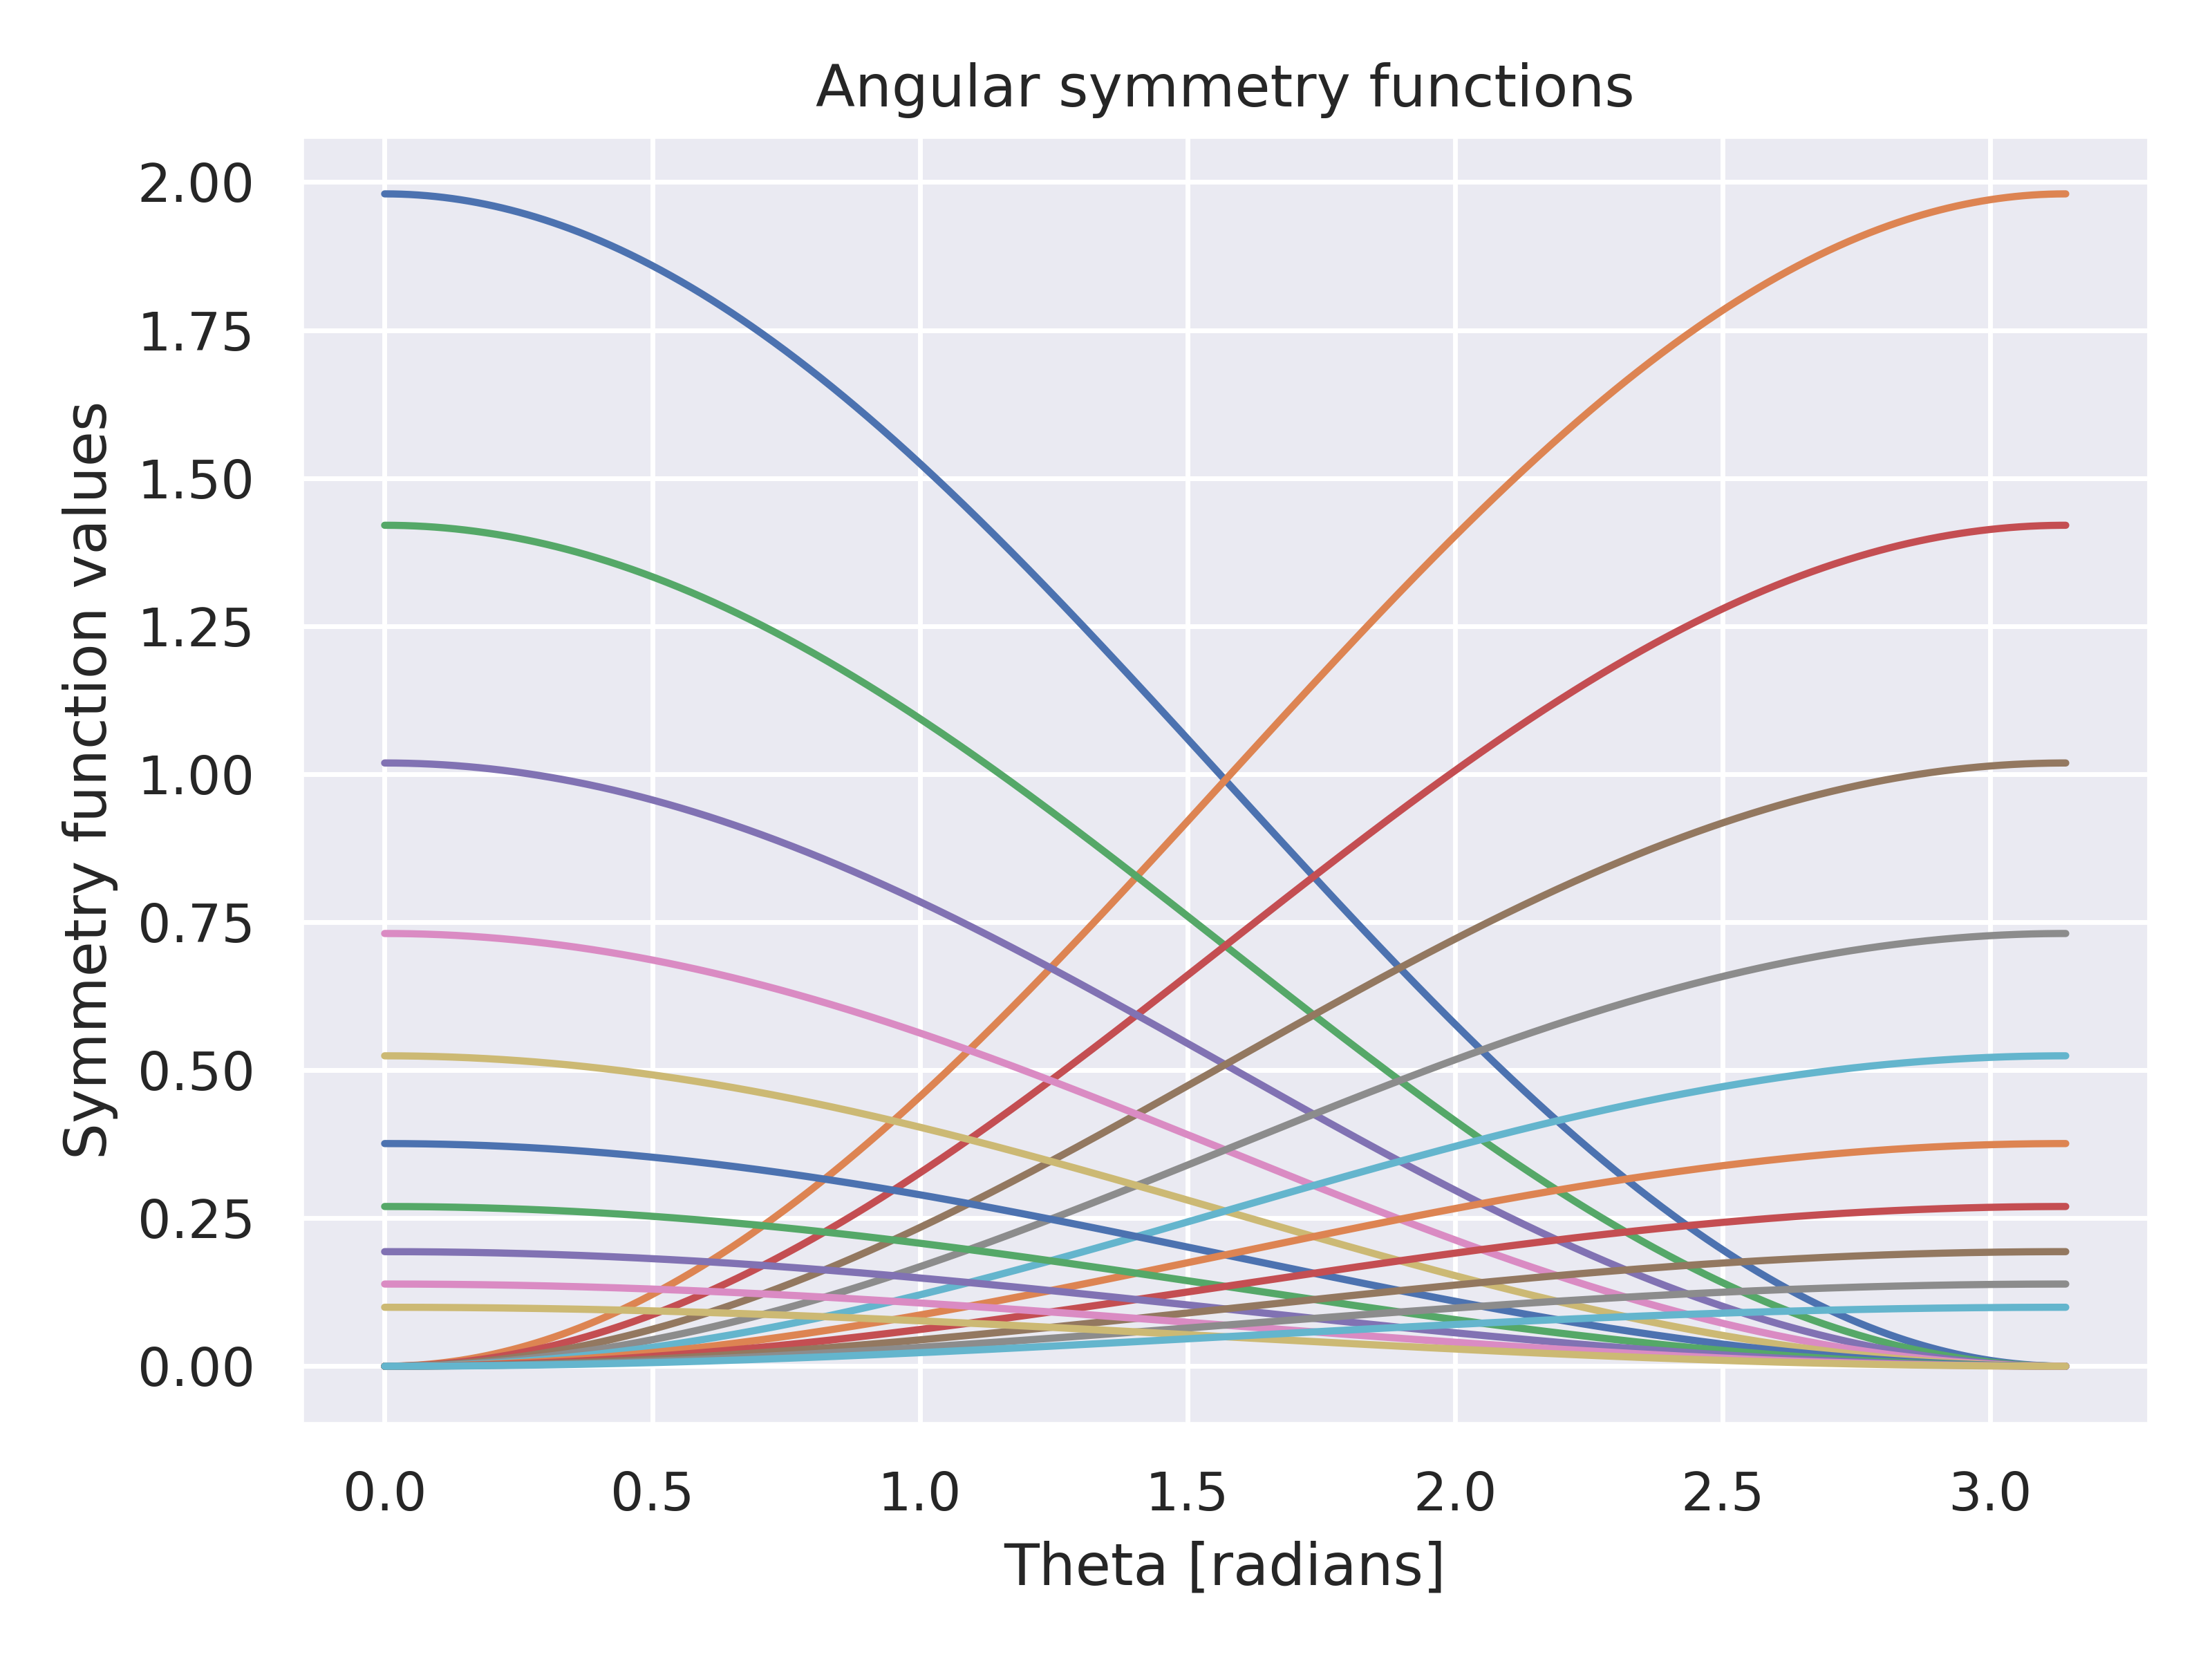
\includegraphics[width=\textwidth]{Selected_ang.png}
      \caption{Angular symmetry functions.}
    \label{fig:f2}
  \end{subfigure}
\end{adjustbox}
    \caption{Selected symmetry function set used for parameter search.
    Radial functions are plotted with radial distribution function.}
    \label{fig:selected}
\end{figure}

\subsection{Force training}
When training the neural networks we have the choice of whether
to incorporate the forces into our loss function, or only fit
the neural network to the potential energy. By default, unless
we have access to a per-atom energy every configuration is labeled
with only a single number for a potentially large number of atoms,
which limits the improvement in loss metrics for every epoch,
and the final result. If instead we incorporate the forces into the
loss we have potentially $3N + 1$ labels for every epoch,
which provides a lot more information for weight updates.
In the previous chapter we also showed how adding derivatives to
the loss function could significantly improve the accuracy of the
derivatives. Since the forces determine the trajectories generated
from molecular dynamics we would expect much better
accuracy and numerical stability if we could improve the fit of
the derivatives.
The real drawback is the calculation of the derivatives in the input layer - 
aka the \textit{fingerprintprimes}, of which there are a lot for every coordinate
and input symmetry function - as they consume a lot of disk space,
memory and CPU time.
\par
In order to test the performance of neural networks
we trained with and without forces on the same set of training images.
A system of copper atoms is generated in the face-centered cubic (FCC)
configuration with 4 atoms in the unit cell and $3 \times 3 \times 3$
unit cells for a total of $4 \cdot 3^3 = 108$ atoms. The
atoms are given velocities from the Maxwell-Boltzmann distribution
corresponding to a temperature of 500 Kelvin. The potential we will
be using is the Effective Medium Theory (EMT), which has a very
fast Fortran implementation in the ASE software package\footnote{
\url{https://wiki.fysik.dtu.dk/asap/asap}}.
The training trajectory is ran for $5 \cdot 10^4$ steps with
a timestep of $\Delta t = 5$ femtoseconds and written to file every 100 steps
for a total of 500 atomic configurations. The test trajectory is
integrated for $1 \cdot 10^4$ steps for a total of 100 atomic configurations.

\begin{figure}[H]
\begin{adjustbox}{max width=1.2\linewidth,center}
\centering
  \begin{subfigure}[b]{0.55\textwidth}
      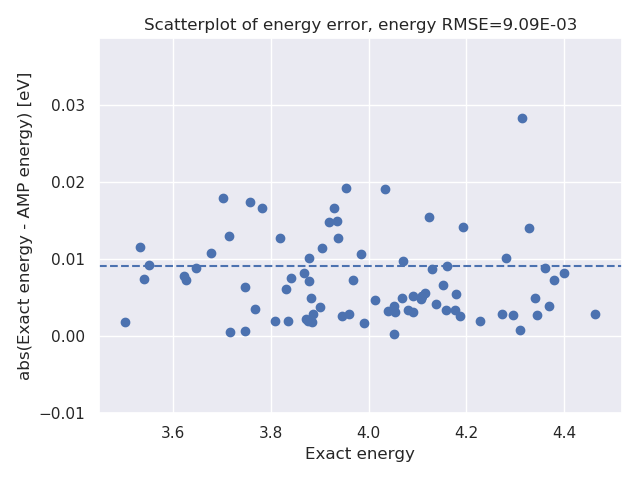
\includegraphics[width=\textwidth]{energy_noforcetrain.png}
      \caption{Energy error.}
    \label{fig:f1}
  \end{subfigure}
  \hfill
  \begin{subfigure}[b]{0.55\textwidth}
      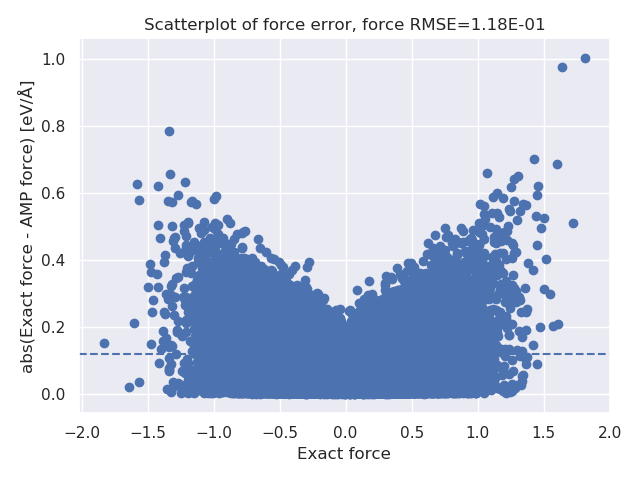
\includegraphics[width=\textwidth]{force_noforcetrain.png}
      \caption{Force component error.}
    \label{fig:f2}
  \end{subfigure}
\end{adjustbox}
\caption{Energy and force component absolute errors and root mean
    squared errors without force training.}
    \label{fig:noforcetrain}
\end{figure}

\begin{figure}[H]
\begin{adjustbox}{max width=1.2\linewidth,center}
\centering
  \begin{subfigure}[b]{0.55\textwidth}
      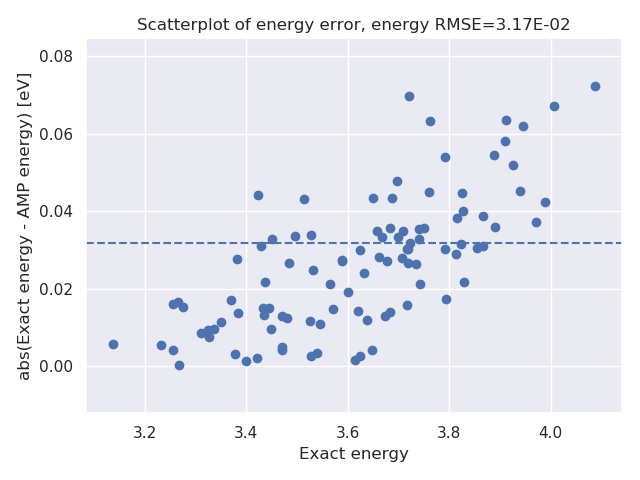
\includegraphics[width=\textwidth]{energy_forcetrain.png}
      \caption{Energy error.}
    \label{fig:f1}
  \end{subfigure}
  \hfill
  \begin{subfigure}[b]{0.55\textwidth}
      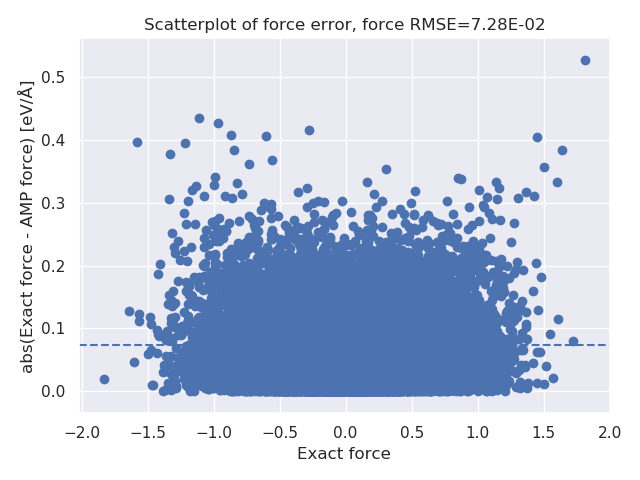
\includegraphics[width=\textwidth]{force_forcetrain.png}
      \caption{Force error.}
    \label{fig:f2}
  \end{subfigure}
\end{adjustbox}
\caption{Energy and force component absolute errors and root mean squred
    errors with force training.}
    \label{fig:forcetrain}
\end{figure}

In figure \ref{fig:noforcetrain} we have created a scatterplot
of the energies and force components vs the absolute error after training without
forces, and labeled the plots with the energy and force RMSEs.
We observe that the potential energies can achieve fairly
low error values of approximately 0.01 to 0.03 eV, and the
result does not depend very much on the value of the exact potential
energy.
The force error however is approximately an order of magnitude
larger, which echoes some of the concerns raised in the previous
chapter with fitting derivatives. The force errors produced by the neural
also appear to be increasing as we move away from zero.
\par
In figure \ref{fig:forcetrain} we have a scatterplot of energies
and force components generated from a force-trained neural network
with a force loss coefficient of $0.1$.
While the error in the potential energy is now approximately 3.5 times higher,
the error in the forces is now about $60 \%$ smaller.
This is arguably a good tradeoff, since the force error matters
much more for long molecular dynamics trajectories, and will make
any simulation requiring large amounts of data more stable.
However, force training is as mentioned much costlier in terms
of memory and CPU hours. Instead of training with forces on the full
set of images, we instead suggest training on a large amount of configurations
with only the energies (and arguably a small amount of atoms, since
the ratio of fingerprints to labels is higher), and subsequently training
with forces on a smaller set of images in order to improve the force fit,
at some cost to the energy fit.

\subsection{Activation, hidden layers}
In order to test different network architectures
we test different choices of the activation functions, and the number
of hidden layers and nodes.
At our chosen range of values, we do not expect a 
large variation in the performance.
Since we do not have a large set of input parameters, we do not expect
a large amount of nodes and hidden layers is required, as this would
only increase the training time,
and larger neural networks with a large amount of hidden layers
might be expected to overfit the training data and generalize poorly.
In the paper Efficient Backprop by \parencite[Lecun et al.]{
lecun2012efficient} the authors suggest that the hyperbolic
tangent outperforms the sigmoid, since the derivatives
are larger, which provides more efficient training.
The hyperbolic tangent is somewhat more computationally costly,
however this is not a big consideration for our neural networks
overall, since they are quite small and can be evaluated
relatively fast.
Inputs should generally be either standardized or scaled, 
as discussed in chapter \ref{chap:optimization},
as these activation functions cannot sufficiently distinguish
large inputs ($\tanh(1000) \approx \tanh(10000)$).
AMP rescales inputs to the range $\left[-1, 1\right]$,
which should be appropriate for both activation functions.
To test different architectures a copper system of $4 \cdot 2^3 = 32$
atoms is generated and integrated for $8 \cdot 10^4$ steps
with a timestep of $\Delta t = 5.0$ femtoseconds
and written to file every 100 steps for a total of 800 training images.
By the same procedure we also obtain 200 test images.
The velocities are generated
according to a Maxwell-Boltzmann distribution with a temperature
of 500 Kelvin. The results are shown in table \ref{table:act-hidden}.
The network is trained only on energies, while for the test set
we calculate the energy and force root mean squared errors (RMSEs).

\begin{table}[H]
\centering
\begin{tabular}{lrr}
\toprule
Activation/Hidden layers &  Energy RMSE &  Force RMSE \\
\midrule
               tanh-[10] &     1.78E-03 &    2.67E-01 \\
               tanh-[20] &     1.83E-03 &    1.80E-01 \\
               tanh-[30] &     1.71E-03 &    5.71E-01 \\
               tanh-[40] &     1.81E-03 &    3.17E-01 \\
           tanh-[10, 10] &     1.73E-03 &    7.71E-02 \\
           tanh-[20, 10] &     1.65E-03 &    3.95E-01 \\
           tanh-[30, 10] &     1.83E-03 &    3.68E-01 \\
           tanh-[40, 40] &     1.87E-03 &    3.42E-01 \\
            sigmoid-[10] &     4.58E-03 &    8.83E-02 \\
            sigmoid-[20] &     3.52E-03 &    1.25E-01 \\
            sigmoid-[30] &     4.72E-03 &    7.27E-02 \\
            sigmoid-[40] &     5.05E-03 &    6.19E-02 \\
        sigmoid-[10, 10] &     3.07E-03 &    2.38E-01 \\
        sigmoid-[20, 10] &     4.89E-03 &    9.93E-02 \\
        sigmoid-[30, 10] &     4.74E-03 &    9.22E-02 \\
        sigmoid-[40, 40] &     4.09E-03 &    7.37E-02 \\
\bottomrule
\end{tabular}
\caption{Training defaults}
\label{table:act-hidden}
\end{table}

From the results we can see that the number of hidden layers
and nodes of the network does not significantly influence the result.
The hyperbolic tangent clearly
outperforms the sigmoid for all sizes in the case of the energy,
while the sigmoid appears to outperform when it comes to the forces.
This is likely because we have not trained the network with force losses,
which means the tangent is better able to fit the energy, and this
degrades somewhat the performance on the forces.
For the hyperbolic tangent with $\left[10, 10\right]$ we are able
to achieve a low energy and force error, and we have seen this result
consistently.
This implies that this size and activation strikes an appropriate balance
between the training epochs required and overfitting, and we have settled
on this architecture for the remainder of the thesis.
However, it remains to be seen if a larger network trained for longer
could outperform the smaller models.

\subsection{Cutoff radius}
The cutoff radius defines the boundary outside of which no interactions
between atoms take place, and the magnitude of the interactions
which take place within. We therefore expect it to have a reasonable
effect on the final result. Ideally we might like all atoms to interact,
as they plausibly do in the real world.
However, since the cutoff radius defines a sphere
with a volume $V \propto R_c^3$, the average number of neighbors and therefore
calculations increases substantially with the cutoff radius.
This means there is a tradeoff
between the accuracy and speed when calculating fingerprints and
fingerprint derivatives, with substantial CPU and memory cost the
larger the cutoff radius.
Accuracy may also be impacted if any
atom interacts with an atom which in actuality does not have a substantial
energy and force contribution.
In figure \ref{fig:copper-rdf} we have plotted the radial distribution
function of copper atoms governed by the EMT potential, together
with the polynomial cutoff function with $\gamma = 5.0$.
The radial distribution function is scaled to $1$ in order to compare
with the cutoff function.
The radial distribution function is highly peaked at $R \approx 2.5, 4.5$,
with smaller peaks as the radial distance grows.
This may justify a fairly small cutoff radius, but it is not clear
how large the cutoff sphere should be until we have examined the results
on the test set.
It is nevertheless reasonable to assume a cutoff between 4 and 8 Angstrom
would perform well, without sacrificing too much accuracy.

\begin{figure}[H]
    \centering
    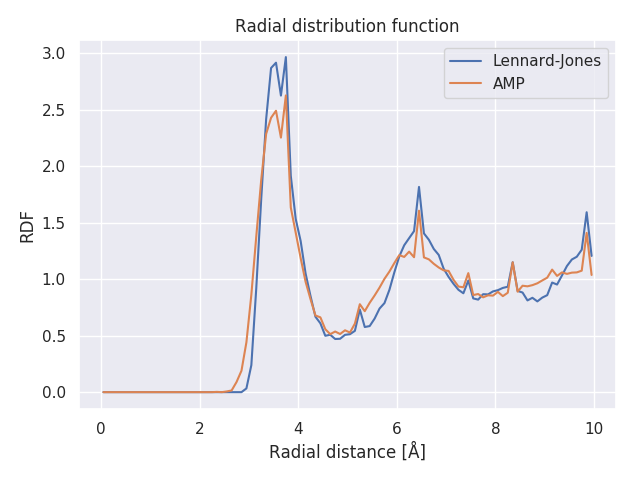
\includegraphics[width=\textwidth]{rdf.png}
    \caption{Radial distribution function of copper atoms
        governed by the EMT potential.}
    \label{fig:copper-rdf}
\end{figure}

We will be comparing the cosine and polynomial cutoffs at different
cutoff radii to test whether one outperforms the other.
As in the previous section we produce a system with 32 atoms, with
800 training configurations and 200 test configurations. The network
is only trained on the energy, since this is substantially cheaper,
and then the network is evaluated on the energy and force RMSE
on the test set. The results are presented in table \ref{table:cutoffs}.

\begin{table}[H]
\centering
\begin{tabular}{lrr}
\toprule
     Cutoff &  Energy RMSE &  Force RMSE \\
\midrule
     Cosine-2.0 &     2.18E-01 &    4.57E-01 \\
 Polynomial-2.0 &     2.18E-01 &    4.57E-01 \\
     Cosine-3.0 &     5.08E-03 &    3.96E-01 \\
 Polynomial-3.0 &     4.85E-03 &    4.12E-01 \\
     Cosine-4.0 &     1.34E-03 &    1.57E-01 \\
 Polynomial-4.0 &     1.21E-03 &    1.42E-01 \\
     Cosine-5.0 &     7.39E-04 &    2.05E-01 \\
 Polynomial-5.0 &     9.34E-04 &    1.91E-01 \\
     Cosine-6.0 &     1.99E-03 &    2.68E-01 \\
 Polynomial-6.0 &     2.42E-03 &    3.84E-01 \\
     Cosine-7.0 &     4.46E-03 &    2.04E-01 \\
 Polynomial-7.0 &     7.71E-03 &    1.18E-01 \\
     Cosine-8.0 &     6.40E-03 &    2.63E-01 \\
 Polynomial-8.0 &     1.05E-02 &    3.41E-01 \\
\bottomrule
\end{tabular}
\caption{Cutoffs}
\label{table:cutoffs}
\end{table}

From the energy RMSEs we can see that the intermediate values of the
cutoff produce the lowest values. This may hint at some kind
of overfitting on the training set,
such that better values are obtained by considering fewer atoms more strongly.
The intermediate values also
seem to produce somewhat lower values of the force RMSE,
of which the lowest is the polynomial with a cutoff of 7 Ångstrøm.
We do not find a substantial difference between the polynomial
and cosine cutoff functions, and these results indicate that not
much is to be gained by choosing one over the other.
We do note that there is a substantial
stochastic element in these tests, and also that longer training
periods may have produced more substantial differences, but
training is costly in terms of CPU time.
For the remainder
of this thesis we settled on the polynomial with a cutoff of 5 Ångstrøm,
while the cosine may have performed just as well.

\subsection{Symmetry functions}\label{chap:symmetry-functions}
The symmetry functions determine the local environment of every atom,
which is then fed to and backpropagated through a neural network
to produce the potential energy and forces,
and should in theory have substantial impact on the final results.
The authors of AMP suggest through experience that the most important
factors are the quality of data, the cutoff radius and the symmetry functions\footnote{
    \href{https://listserv.brown.edu/cgi-bin/wa?A2=AMP-USERS;52062bd3.1810}{
        AMP mailing list}}.
The symmetry functions should cover both the radial and angular
environment of the atoms in the system we are trying to learn from.
They should also be distinguishable in order for the neural network
to be able to separate different chemical environments.
J{\"o}rg Behler writes in his article on neural network potential
energy surfaces \parencite[Behler]{behler2011neural}
that the symmetry functions should describe the structures uniquely,
and not be too highly correlated.
In their article on Weighted Atom-Centered Symmetry Functions
\parencite[Gastegger et al.]{gastegger2018wacsf} suggest that uncentered
aka shifted radial symmetry functions perform better than symmetry functions
centered at $R_s = 0$, since these offer better coverage of the radial space.
They also suggest that this is not the case for angular symmetry functions,
since they are products of multiple gaussians which narrows their range
of values. 
Furthermore they suggest that for angular symmetry functions
the parameter $\zeta$ should be limited to values of 1 or 2,
and they demonstrate that increasing this parameter narrows
the functions to a smaller range of angles close to the maxima
(i.e. 0 or 90 degrees).
We follow some of their suggestions and use a combined set of
centered and uncentered radial functions. 
In the introduction to this chapter we defined a method
for constructing the set of symmetry functions, with the parameters
being the number of radial functions, angular functions, zetas
and the type of angular function.
To find the optimal set
we perform tests of the energy and force RMSE while varying the
number of radial and angular symmetry functions, and testing
whether the G4 or G5 type of angular functions performs noticeably
better than the other type.
The results are presented in table \ref{table:symmetry}.
The first parameter is the number of radial $\eta$'s,
the second is the number of angular $\eta$'s and the third
is the number of $\zeta$ values.

\begin{table}[H]
\centering
\begin{tabular}{lrr}
\toprule
Symmetry function &  Energy RMSE &  Force RMSE \\
\midrule
          Default &     8.07E-02 &    6.99E+00 \\
      Gs-4-8-1-G4 &     2.55E-03 &    8.54E-02 \\
      Gs-4-8-1-G5 &     3.11E-03 &    5.26E-02 \\
      Gs-5-9-1-G4 &     2.08E-03 &    2.42E-01 \\
      Gs-5-9-1-G5 &     2.65E-03 &    1.36E-01 \\
     Gs-6-10-1-G4 &     1.88E-03 &    6.60E-02 \\
     Gs-6-10-1-G5 &     2.14E-03 &    1.99E-01 \\
     Gs-7-11-1-G4 &     1.68E-03 &    2.98E-01 \\
     Gs-7-11-1-G5 &     1.96E-03 &    4.54E-02 \\
     Gs-8-12-1-G4 &     1.75E-03 &    1.38E-01 \\
     Gs-8-12-1-G5 &     1.66E-03 &    8.30E-02 \\
     Gs-9-13-1-G4 &     1.70E-03 &    1.00E-01 \\
     Gs-9-13-1-G5 &     2.58E-03 &    2.08E-01 \\
    Gs-10-14-1-G4 &     1.52E-03 &    4.30E-02 \\
    Gs-10-14-1-G5 &     2.58E-03 &    1.70E-01 \\
    Gs-10-14-2-G4 &     1.18E-03 &    1.71E-01 \\
    Gs-10-14-2-G5 &     1.92E-03 &    2.04E-01 \\
\bottomrule
\end{tabular}
\caption{Symmetry functions}
\label{table:symmetry}
\end{table}

From these results we observe that the energy errors are marginally
improved by increasing the number of symmetry functions, though the
errors may be increasing at the upper end. This may indicate
that an intermediate mix of symmetry functions offers appropriate
coverage of the radial and angular space, while too many symmetry
functions makes environments difficult to distinguish.
The type of angular function seems to matter, but is dependent
on the mix of symmetry functions, as one type outperforms the other
dependent on the composition.
We speculate that the force errors generally improve as we increase
the number of symmetry functions, as forces represent the change in energy
from a small perturbation of the position of a single atom,
and this may be better represented by having a larger number of functions
sensitive to this change.
Our method of generating symmetry function markedly outperforms
the AMP default symmetry functions, which suggest that we exercise
some care when selecting the symmetry function set.
As for the number of zetas, we only test two values with
$\zeta = 1, 2$, thus doubling the number of angular symmetry functions,
and this does not seem to significantly improve the error rate,
though we may have found larger differences if this was tested more.

\subsection{Overfitting and regularization}
Overfitting describes the phenomenom whereby statistical learning methods
that perform well on a training set perform poorly on the test set,
and indicates poor generalization.
In order to guard against overfitting we try to ensure that the
neural network architecture is not too complicated, and typically
we add a term to the loss function proportional
to the size of the weights and biases,
as this ensures that no weight can be adjusted to arbitrary size
to fit the training dataset.
In order to test whether the neural network is overfitting the training
data we generate the same configurations as before and vary
the value of the regularization proportionality term $\lambda$.
Once the neural networks have been trained we evaluate their
performance on the test set. The results are shown in table \ref{table:overfit}.

\begin{table}[H]
\centering
\begin{tabular}{lrr} 
\toprule
Regularization &  Energy RMSE &  Force RMSE \\
\midrule
     1.00e+00 &     9.36E-02 &    3.92E-01 \\
     1.00e-01 &     9.33E-02 &    3.92E-01 \\
     1.00e-02 &     9.34E-02 &    3.92E-01 \\
     1.00e-03 &     9.34E-02 &    3.92E-01 \\
     1.00e-04 &     3.35E-02 &    2.97E-01 \\
     1.00e-05 &     9.86E-03 &    1.63E-01 \\
     1.00e-06 &     5.14E-03 &    1.20E-01 \\
     1.00e-07 &     2.29E-03 &    1.11E-01 \\
     1.00e-08 &     1.52E-03 &    3.02E-01 \\
     1.00e-09 &     1.32E-03 &    2.35E-01 \\
\bottomrule
\end{tabular}
\caption{Regularization parameter search.}
\label{table:overfit}
\end{table}

From these results we see that for values of the regularization parameter
that are too large, the regularization is too punishing,
and the training is not able to find any appropriate minima.
The errors seem to improve as the regularization decreases,
while the force errors rise slightly as the regularization continues
to decrease.
Since we have such a small neural network, large values of the regularization
are too punishing, while small values are equivalent to no regularization,
and overfitting is not prevented. 
From these results we do not find much evidence of overfitting, but
they may suggest some small regularization is appropriate for
optimal generalization performance.

\subsection{Sampling and scaling}
In order for the neural network to learn patterns from data
the data needs to be of high quality, and atomic configurations
should be sufficiently distinguishable while being representative
of the underlying distribution. Neural networks typically perform
poorly or unexpectedly on unseen data, in addition to being data-hungry
requiring fairly large amounts of data in order to train well
over many epochs.
One approach to learning atomic configurations might be to generate
random configurations (not too closely spaced) and calculate energy
and forces from these using a suitable calculator. However, this
phase space of configurations would be enormous using only a few particles,
and we would encounter many highly unlikely configurations.
Since we want to train the neural network to perform molecular dynamics,
the obvious solution is to sample configurations from molecular dynamics
trajectories. However, these configurations are (mostly) in equilibrium, with
relatively small forces, and thus the network might struggle if
it encounters smaller distances between atoms.
In their paper on fitting potential energy surfaces using neural networks,
\parencite[Pukrittayakamee et al.]{pukrittayakamee2009simultaneous}
suggest using a variable time interval dependent on the maximum acceleration:

\begin{equation}
    \tau = 
    \begin{cases}
        \text{trunc}[\alpha / a_{max}]\Delta t & \text{trunc}
        [\alpha / a_{max}] > 0, \\
        \Delta t & \text{trunc}
        [\alpha / a_{max}] = 0,
    \end{cases}
\end{equation}

where $\Delta t$ is a minimum time interval and $\alpha$ is a parameter
which must be determined empirically.
The rationale behind this is that we will sample more from
areas where the forces are large, while skipping areas
where the forces are small.
In our experiments using this algorithm (slightly modified)
we find that appropriate choices of $\Delta t$ and $\alpha$
can broaden the distribution of force somewhat.
However it does not add a substantial amount of larger forces, since
these are simply not present in equilibrium.
Other sampling algorithms have been suggested, for example iteratively
pruning a large data set of images by removing images where
the errors are not very large, and then retraining on the pruned datasets
until we are satisfied with the result.
One can also check for images where new values of the fingerprints
are encountered and add these to the training set, or checking
images for large overall values of the feature vector. 
Behler in his review\cite{behler2011neural} on neural network potentials
suggests that sampling from equilibrium states may leave holes
in the potential energy surface, and suggests a few ways of dealing
with this sampling problem.
However, we have not had time to test these different methods.
Other methods such as metadynamics\footnote{
\url{https://parrinello.ethz.ch/research/metadynamics.html}}
have seen increasing application and there are now numerous implementations
available such as PLUMED \footnote{\url{https://www.plumed.org/}}.
In general, though sampling has not been studied closely in this thesis,
an increase in high quality data is an increase in neural network
performance, both for electronic structure calculations
and for other applications.
Neural networks are known as data-hungry, and typically require
a large amount of data to perform well and also scale well
with the number of data points. 
In order to test the accuracy as we add data points
we train a neural network on progressively larger sets of images generated 
from molecular dynamics, and evaluate them on a test set.
The results are shown in table \ref{table:images}.

\begin{table}[H]
\centering
\begin{tabular}{lrr}
\toprule
Number of images &  Energy RMSE &  Force RMSE \\
\midrule
             10 &     1.33E-01 &    6.84E-01 \\
             20 &     2.51E-02 &    3.10E-01 \\
             50 &     1.07E-02 &    1.32E-01 \\
            100 &     5.58E-03 &    3.03E-01 \\
            200 &     2.00E-03 &    1.81E-01 \\
            500 &     1.78E-03 &    9.79E-02 \\
           1000 &     1.82E-03 &    3.07E-01 \\
           2000 &     1.58E-03 &    1.06E-01 \\
           5000 &     1.36E-03 &    1.62E-01 \\
          10000 &     1.42E-03 &    9.61E-02 \\
\bottomrule
\end{tabular}
    \caption{Neural network accuracy as a function
        of the number of images.}
    \label{table:images}
\end{table}

From these results we see that the energy RMSE scales favorably as
the number of images available increase, and the force RMSE decreases
as well, though not as systematically, due to stochasticity and
the fact that the networks have not been trained on force.
However, the gain in performance tails off after approximately 500 data points,
which suggests that there is not much more to be gained from
adding more configurations.
Instead of sampling more configurations from equilibrium, we may
be better served by looking at alternative sampling algorithms,
sampling at higher or varying temperatures to introduce larger
forces into the trajectory or introducing force training.
